% =====================================================================
%  IEEE-STYLE CONFERENCE REPORT TEMPLATE  (self-contained)
%  MLE-AI-201 Machine Learning -- Final Project
%
%  This template MIMICS the IEEE two-column conference look using only
%  standard LaTeX packages. It does NOT depend on IEEEtran.cls, so it
%  compiles anywhere (tectonic, pdflatex, Overleaf) with nothing extra.
%
%  Build:   tectonic report.tex      (recommended)
%     or:   pdflatex report.tex ; pdflatex report.tex
% =====================================================================
\documentclass[10pt,twocolumn,a4paper]{article}

% ---- Geometry: IEEE-like margins / two narrow columns ----------------
\usepackage[a4paper,top=0.75in,bottom=1.0in,left=0.68in,right=0.68in,columnsep=0.25in]{geometry}

% ---- Times-like font (standard, ships with every TeX distro) ---------
\usepackage{mathptmx}          % Times text + math
\usepackage[T1]{fontenc}
\usepackage[utf8]{inputenc}    % allows accented / Azerbaijani chars

% ---- Common, dependency-free packages --------------------------------
\usepackage{graphicx}
\usepackage{amsmath,amssymb}
\usepackage{booktabs}
\usepackage{array}
\usepackage{titlesec}
\usepackage{caption}
\usepackage{cite}
\usepackage[hidelinks]{hyperref}
\usepackage{url}

% ---- IEEE-style section headings -------------------------------------
\renewcommand{\thesection}{\Roman{section}}
\renewcommand{\thesubsection}{\Alph{subsection}}
\titleformat{\section}[block]{\centering\normalsize\scshape}{\thesection.}{0.5em}{}
\titleformat{\subsection}[block]{\normalsize\itshape}{\thesubsection.}{0.5em}{}
\titlespacing*{\section}{0pt}{1.4ex plus 1ex minus .2ex}{1ex}
\titlespacing*{\subsection}{0pt}{1.0ex plus 1ex minus .2ex}{0.6ex}

% ---- Abstract / Index-Terms in the IEEE boldface-dash style ----------
\newcommand{\abstractkw}[1]{\noindent\textbf{\textit{#1}}}

\captionsetup{font=small,labelsep=period}
\setlength{\parindent}{1em}

% =====================================================================
\begin{document}

% ------------------------- TITLE BLOCK --------------------------------
\twocolumn[
  \begin{@twocolumnfalse}
  \begin{center}
    {\LARGE\bfseries Bina.az Price Prediction:\\From-Scratch Trees and a Pegasos SVM\par}
    \vspace{1.2em}
    % Authors: Surname, Given name --- alphabetical by surname.
    {\large
      Shukurlu, Nural\par}
    \vspace{0.5em}
    {\itshape MLE-AI-201 Machine Learning, AI Academy --- Cohort II\par}
    \vspace{1.4em}
  \end{center}
  \begin{quote}
    \small
    \abstractkw{Abstract---}%
    I predict apartment prices from messy bina.az sale listings and a
    derived premium/standard price tier. Both core models are my own
    NumPy code: a decision tree (Gini/entropy/MSE, exact split search)
    and a linear SVM trained with Pegasos sub-gradient descent, plus a
    random-Fourier-feature extension. On 62,673 cleaned listings my
    tree reaches test RMSE 368k~AZN ($R^2{=}0.55$) and tier F1 0.918,
    matching the tuned scikit-learn tree (RMSE 378k, F1 0.919); my
    Pegasos SVM reaches F1 0.832 (AUC 0.920) against 0.854 for
    \texttt{SGDClassifier}. Prices are heavy-tailed so the regressor is
    trained on $\log(\mathrm{price})$. Code and figures reproduce with
    one command, \texttt{python -m src.run\_all}:
    \href{https://github.com/nuralnetworks/bina-az-price-prediction}{\texttt{github.com/nuralnetworks/bina-az-price-prediction}}
    (tag \texttt{v1.0-final}).

    \vspace{0.6em}
    \abstractkw{Index Terms---}decision tree, support-vector machine,
    Pegasos, regression, classification, real-estate price prediction.
  \end{quote}
  \vspace{1.0em}
  \end{@twocolumnfalse}
]

% =====================================================================
\section{Introduction}
Bina.az is Azerbaijan's largest property marketplace, and its listing
dump is genuinely messy: mixed types, Azerbaijani free text, missing
fields, scrape duplicates and heavy-tailed prices. I turn it into two
tasks: (A) regression of the sale price and (B) classification of a
price tier (premium vs.\ standard, split at the training median of
213{,}000~AZN). My contributions: (i) a documented cleaning pipeline
with leakage removal; (ii) a from-scratch decision tree for both tasks;
(iii) a from-scratch Pegasos SVM with a Fourier-feature extension;
(iv) a matched, seeded benchmark against scikit-learn with uncertainty.

\section{Related Work / Background}
Classification trees split by impurity decrease,
$G{=}1{-}\sum_k p_k^2$, $H{=}{-}\sum_k p_k\log_2 p_k$,
$IG{=}I{-}\sum_c \frac{N_c}{N}I(c)$, and regression trees by variance
reduction~\cite{pegasos}. The soft-margin SVM minimises the regularised
hinge primal, solved here with the Pegasos stochastic sub-gradient
method~\cite{pegasos} instead of a QP/SMO solver.

\section{Data and Preprocessing}
The dump holds 100{,}775 raw rows and 51 columns. I deduplicate on the
canonical listing URL (28\% are rescrapes), coerce prices and areas to
numeric, parse \textit{Saha} (145~m\textsuperscript{2},
\textit{Mertebe} (7~/~9 $\to$ floor and
total floors) and \textit{Torpaq sahesi} (1.3~sot), and drop
rows with price outside [10k, 15M]~AZN, area outside [10, 3000]~m\textsuperscript{2},
or coordinates outside the Absheron box. All currencies are AZN, so no
conversion is needed. This leaves 62{,}673 rows and 43 features:
13 numeric (area, rooms, floor, floors total, land, location, flags)
plus one-hot district (top-15 + other) and deed/repair/mortgage state;
missing floors become $-1$ and missing rooms $0$, so no statistic leaks
across splits. \textbf{Leakage removed:} \texttt{unit\_price} (price per
m\textsuperscript{2}) and \texttt{total\_price} (== price), plus IDs, URLs,
scrape timestamps, owner/shop names and free-text address. The tier
threshold (median 213{,}000~AZN) and all standardisation statistics come
from the training split only. Split: 43{,}869 train / 9{,}402 val /
9{,}402 test (70/15/15, stratified by price quintile); the test tier
balance is 50.1\% premium.

\begin{table}[t]
  \centering
  \caption{Dataset summary after cleaning.}
  \label{tab:data}
  \begin{tabular}{@{}lr@{}}
    \toprule
    Property & Value \\
    \midrule
    Rows (after cleaning)       & 62{,}673 \\
    Features used               & 43 \\
    Train / Val / Test split    & 43869 / 9402 / 9402 \\
    Price-tier balance (\%)     & 50.0 / 50.1 (train/test premium) \\
    \bottomrule
  \end{tabular}
\end{table}

\section{Method}
\subsection{Decision tree (from scratch)}
Exact greedy split search over sorted feature values (candidate
thresholds capped at 255 quantiles for speed), gain
$I{-}(N_L I_L{+}N_R I_R)/N$, recursive growth with
\texttt{max\_depth}, \texttt{min\_samples\_split},
\texttt{min\_samples\_leaf} and \texttt{min\_impurity\_decrease} all
enforced, majority/mean leaves, leaf-frequency \texttt{predict\_proba},
and impurity-decrease importances. Supports Gini, entropy and MSE.
A toy check (1-D, depth-1) reproduces sklearn's split and predictions exactly.

\subsection{Support-vector machine (from scratch)}
\begin{equation}
  J(\mathbf{w},b)=\tfrac{\lambda}{2}\lVert\mathbf{w}\rVert^{2}
  +\tfrac{1}{n}\sum_{i=1}^{n}\max\!\big(0,\,1-y_i(\mathbf{w}^{\top}\mathbf{x}_i+b)\big).
\end{equation}
Pegasos update with $\eta_t{=}1/(\lambda t)$ on standardised features,
objective traced to convergence. Non-linear extension: random Fourier
features ($\Phi(x){=}\sqrt{2/D}\cos(XW{+}b)$, $D{=}500$) approximating
the RBF kernel, chosen because it reuses the same linear solver with a
few lines of code. Margin width $2/\lVert\mathbf{w}\rVert$ and support
points ($y_i f(x_i){\le}1$) are reported.

\section{Experimental Setup}
Task~A metrics: RMSE/MAE/$R^2$ on price (model trained on
$\log(\mathrm{price})$, predictions exponentiated; log-RMSE also given).
Task~B metrics: precision/recall/F1, ROC-AUC and confusion matrix.
Tuning on validation only: tree depths $\{4,6,8,12,16\}$ (+leaf
$\{1,5,20\}$), SVM $\lambda{\in}\{10^{-5}{..}10^{-2}\}$ and RFF
$\gamma{\in}\{0.005,0.02,0.05\}$. Baselines with matched settings:
\texttt{DecisionTreeRegressor/Classifier} and
\texttt{SGDClassifier(hinge)}. Uncertainty: 5-fold CV mean $\pm$ std on
train. Seed 42 everywhere; \texttt{python -m src.run\_all} reproduces
all numbers and figures.

\section{Results}
Final configs (val-chosen): tree-reg depth~12/leaf~5; tree-clf Gini,
depth~12/leaf~1; SVM $\lambda{=}0.01$, RFF $\gamma{=}0.005$.
Table~\ref{tab:results} and Figs.~\ref{fig:price}--\ref{fig:cm} tell a
consistent story: my tree matches sklearn on both tasks (gaps are
tie-breaking/float thresholds), and my Pegasos SVM trails sklearn's
averaged hinge-SGD by 0.02 F1. RFF underperforms the linear SVM here
(0.767 vs.\ 0.832), so the linear model stays my final SVM.

\begin{table}[t]
  \centering
  \caption{Headline results (test set; CV is 5-fold mean $\pm$ std on train).}
  \label{tab:results}
  \small
  \begin{tabular}{@{}lcc@{}}
    \toprule
    Model & Task A (RMSE) & Task B (F1) \\
    \midrule
    My tree     & 368{,}435 & 0.918 (CV $0.911{\pm}0.002$) \\
    My SVM (linear) & n/a & 0.832 (CV $0.832{\pm}0.007$) \\
    My SVM (RFF) & n/a & 0.767 \\
    sklearn tree      & 377{,}891 & 0.919 (CV $0.910{\pm}0.003$) \\
    sklearn SGD hinge & n/a & 0.854 \\
    \bottomrule
  \end{tabular}
\end{table}

\begin{figure}[t]
  \centering
  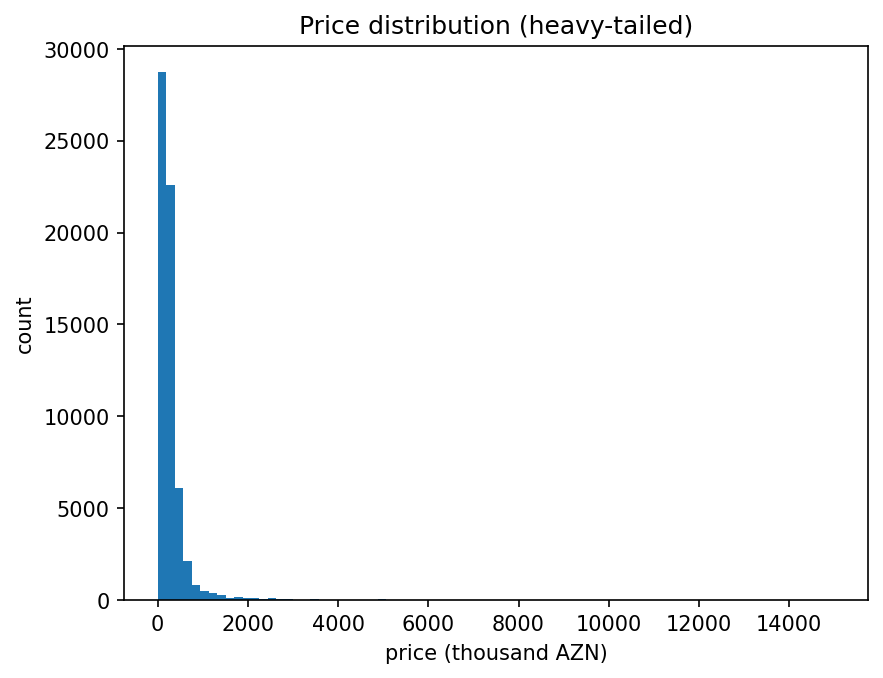
\includegraphics[width=\linewidth]{figures/price_hist.png}
  \caption{Price is heavy-tailed, motivating the $\log(\mathrm{price})$ target.}
  \label{fig:price}
\end{figure}

\begin{figure}[t]
  \centering
  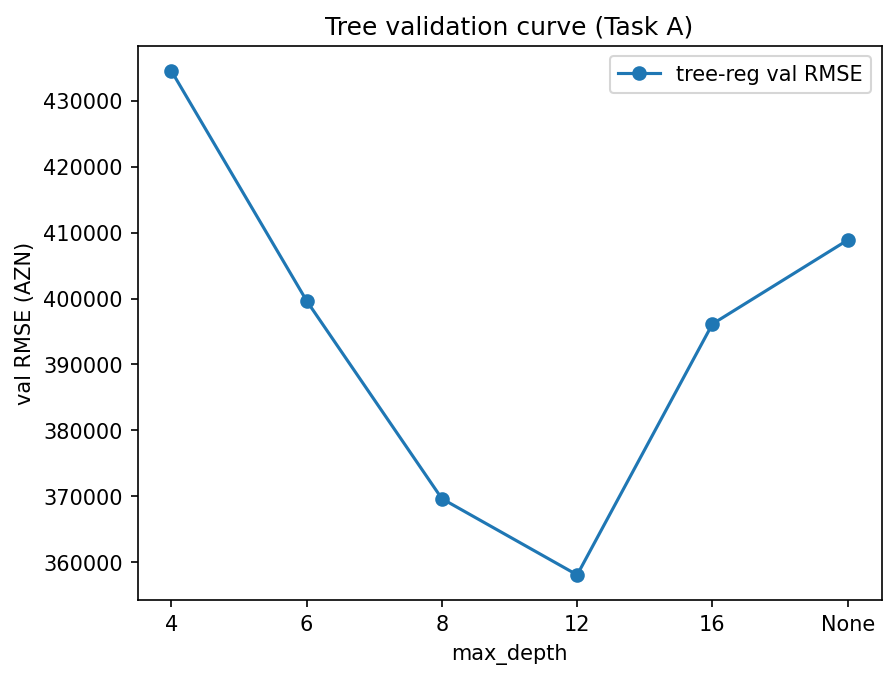
\includegraphics[width=\linewidth]{figures/tree_val_curve.png}
  \caption{Tree validation curve (Task~A): RMSE bottoms at depth 12, then overfits.}
  \label{fig:treeval}
\end{figure}

\begin{figure}[t]
  \centering
  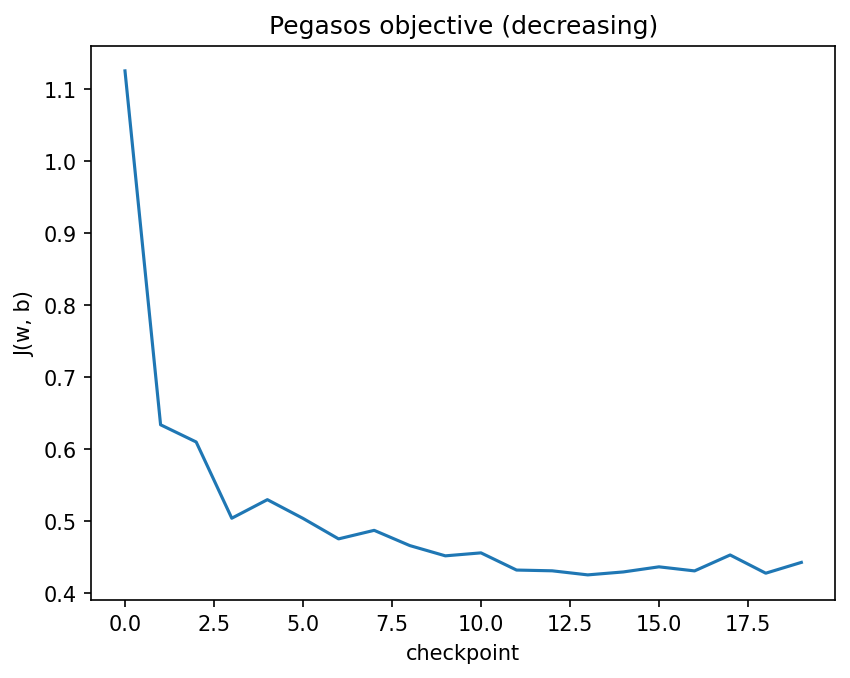
\includegraphics[width=\linewidth]{figures/svm_objective.png}
  \caption{Pegasos objective $J(\mathbf{w},b)$ decreases and settles.}
  \label{fig:svmobj}
\end{figure}

\begin{figure}[t]
  \centering
  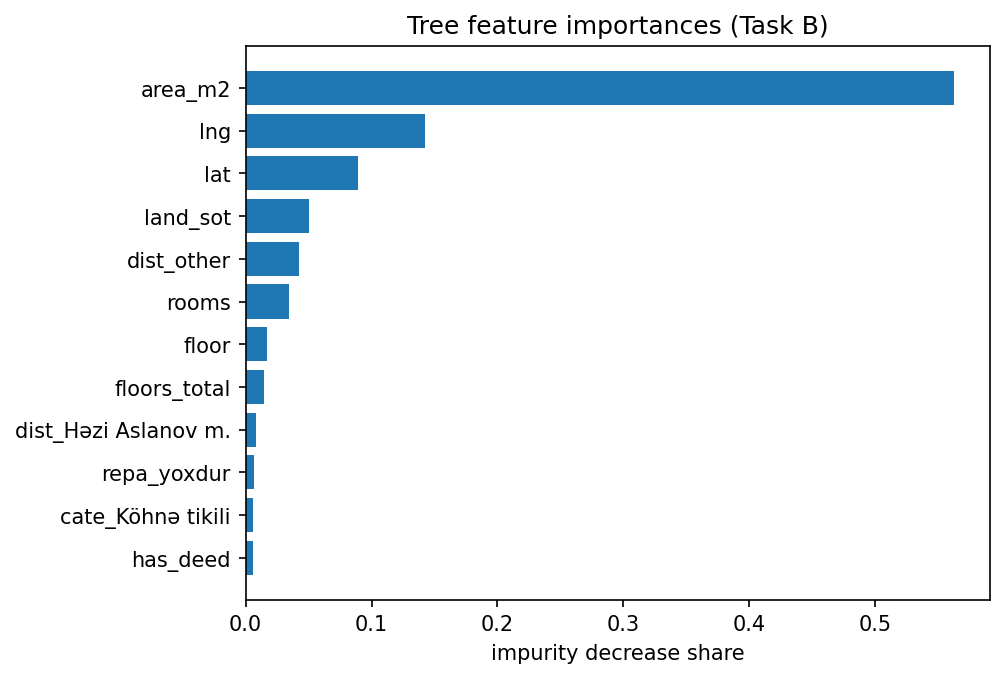
\includegraphics[width=\linewidth]{figures/importance.png}
  \caption{Top tree importances (Task~B): area, location and rooms dominate.}
  \label{fig:imp}
\end{figure}

\begin{figure}[t]
  \centering
  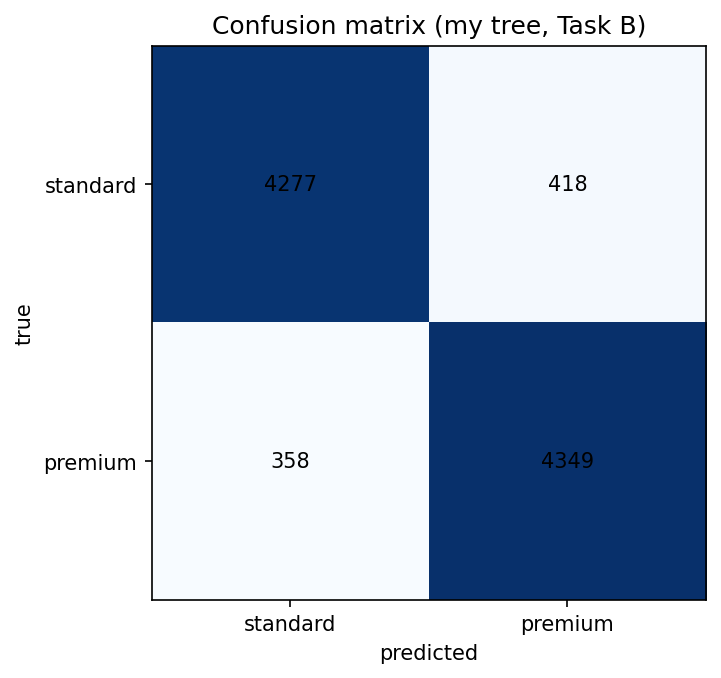
\includegraphics[width=\linewidth]{figures/confusion.png}
  \caption{Confusion matrix, my tree on Task~B test (F1 0.918, AUC 0.955).}
  \label{fig:cm}
\end{figure}

\section{Discussion and Limitations}
Depth~16/unlimited overfits Task~A (val RMSE 396k/409k vs.\ 358k at
depth~12); Gini beats entropy slightly on Task~B (0.918 vs.\ 0.916).
Stronger $\lambda$ widens the realised margin (0.0048 $\to$ 0.73) while
raising the support fraction (0.20 $\to$ 0.41) and val F1, so
$\lambda{=}0.01$ is kept. Errors concentrate on luxury outliers
(RMSE lives there while MAE is 86k) and sparse outskirt districts where
one-hot columns are thin; RFF adds variance without signal on these
already high-dimensional sparse features. Limits: single 70/15/15 split
for headline numbers (CV only on train), no text/image features, and
scrape-time dedup keeps the last snapshot only.

\section{Conclusion}
From-scratch trees match the reference implementation on both tasks and
the Pegasos SVM is competitive with sklearn's hinge-SGD; careful
cleaning and leakage removal matter more than model choice here. Next
would be text features from descriptions and grouped-by-district error
modelling.

\section*{Tools and Acknowledgements}
Data: bina.az sale dump via Kaggle (\texttt{sehriyarmemmedli/binaaz-sale-project}),
downloaded Oct~2026; baselines and CV utilities from scikit-learn;
plots with matplotlib. Report template is the course self-contained
two-column style. Contributions are listed in \texttt{contribution\_report.md}.
The mathematical descriptions, formulas and from-scratch algorithms were
implemented by me with the help of an AI assistant (plus \LaTeX\
formatting); the work itself — design, experiments and analysis — is mine.

% =====================================================================
\begin{thebibliography}{9}
\bibitem{pegasos}
S.~Shalev-Shwartz, Y.~Singer, N.~Srebro, and A.~Cotter,
``Pegasos: primal estimated sub-gradient solver for SVM,''
\emph{Mathematical Programming}, vol.~127, no.~1, pp.~3--30, 2011.
\end{thebibliography}

\end{document}
